\section{Design}

\subsection{Tools and techniques}

\subsubsection{Tools}
\begin{itemize}
	\item \textbf{Github}: the source control platform used during the whole project development. Commit history, auto-generated progress statistics, progress tracking.
	\item \textbf{Visual Studio Code}: editor of choice, syntax highlighting, integrated debugger and unit test executor.
	\item \textbf{virtualenv}: Python environment isolation tool. Separates the development environment from the global machine environment, mitigates indirect permissions, dependencies and version incompatibility issues.
	\item \textbf{pip}: Python package installer. Keeps track of project dependencies, simplifies installation and deployment.
	\item \textbf{Lucidchart}: web-based tool for creation of UML diagrams and drawings. Used for planning and documentation purposes. 
	\item \textbf{pylint}: source-code bug and quality checker for Python following PEP8 style guide {18}. Highlights pure code practises and impose the use of good coding practices.
	\item \textbf{autoDocstring}: Visual Studio code extension for Python comment generation. Help to keep consistent commenting style and contributed to good coding practises.
	\item \textbf{Qt 5 Designer}: easy-to-use graphical user interface tool for designing and building Qt UI for the static part of the application.
\end{itemize}

\subsubsection{Libraries}
\begin{itemize}
	\item \textbf{pytest}: Python unit test framework. Extensively used during the whole prototype development process.
	\item \textbf{jsonpickle}: Third-party Python library used for exporting threat model as structured data.
	\item \textbf{ruamel.yaml}: Third-party Python library used for parsing yaml files. Yaml files were used to describe tools included in the tool set as well as providing 'caching' for the threat model entries. 
	\item \textbf{PyQt5}: a Python binding for a well known Qt v5 cross-platform C++ libraries set. It provides native look across common platforms and is used for the projects visual part. 
\end{itemize}

\subsubsection{Techniques}
\begin{itemize}
	\item \textbf{MVC pattern}
	
	Model-View-Controller architecture is used to separate the application data from it's visualization. Due to the inherited modularity of the project - combination of a threat model and a tool set - two separate instances of MVC pattern are used. 
	
	The first MVC instance is representing the threat model. The overall threat model data object is linked with the parent threat model Controller which contains the narrow purpose Controllers. Each Controller object in the parent Controller is linked to corresponding View object. View objects represent separate parts of threat model GUI. 
	
	The second MVC instance is needed to structure the tool set. There is generic object containing all the seprate penetration tool information. Each independent penetration tool has it's own Model representation. All penetration tools in the tool set have generated graphical user interfaces. These GUI's are created together with linked controllers by the tool Model objects in accordance to the tool data stored in those Models.
	
	\item \textbf{Facade pattern}
	
	Facade pattern is used to hide internal system complexity providing a simpler interface to use. In the project it is used to mask threat model internal relations providing a general "Threat Model" object to work with. The internal structure of a penetration tool object as well as the process of parsing it's configuration data is also encapsulated.
	
	\item \textbf{Interpreter pattern} (just defining language and parsing in recursively)
	
	Interpreter pattern is used while parsing penetration tool configuration files. Complete majority of pen testing tools can be run from the terminal. Unfortunately, various tool syntaxes tend to have fundamental differences. Therefore, one part of configuration parsing process is to interpret unique tool syntax which may also contain recursive patterns.
	
	\item \textbf{Observer pattern}
	
	Qt graphic components can make use of observer pattern to notify linked devices of different events. In Qt this pattern is called "Signal and Slot" mechanism. Signals can be "emitted" in response to system or custom actions and connected functions - Slots (can be enclosed in other objects) will execute in reply. It is used across the application to create dynamically linked and responsive GUI.
	
	\item \textbf{Object pooling}
	
	As the application uses threat pooling technique it supports parallel execution of multiple penetration testing tools. This way application main event loop is separated from individual tool execution.
	
	\item \textbf{Serialization}
	
	Serialization is used to preserve information kept in the threat model between work sessions. Threat modelling projects can be saved, closed and re-opened. Due to the way Python serializes objects the tool set implementation can be altered (e.g. a new version is released) still maintaining compatibility with threat model files created by older software versions.
	
\end{itemize}

\subsection{Application structure}

\subsubsection{High level design}
High level project structure is presented in figure \ref{fig:high-level-struct} below.

\begin{figure}[!htb]
	\center{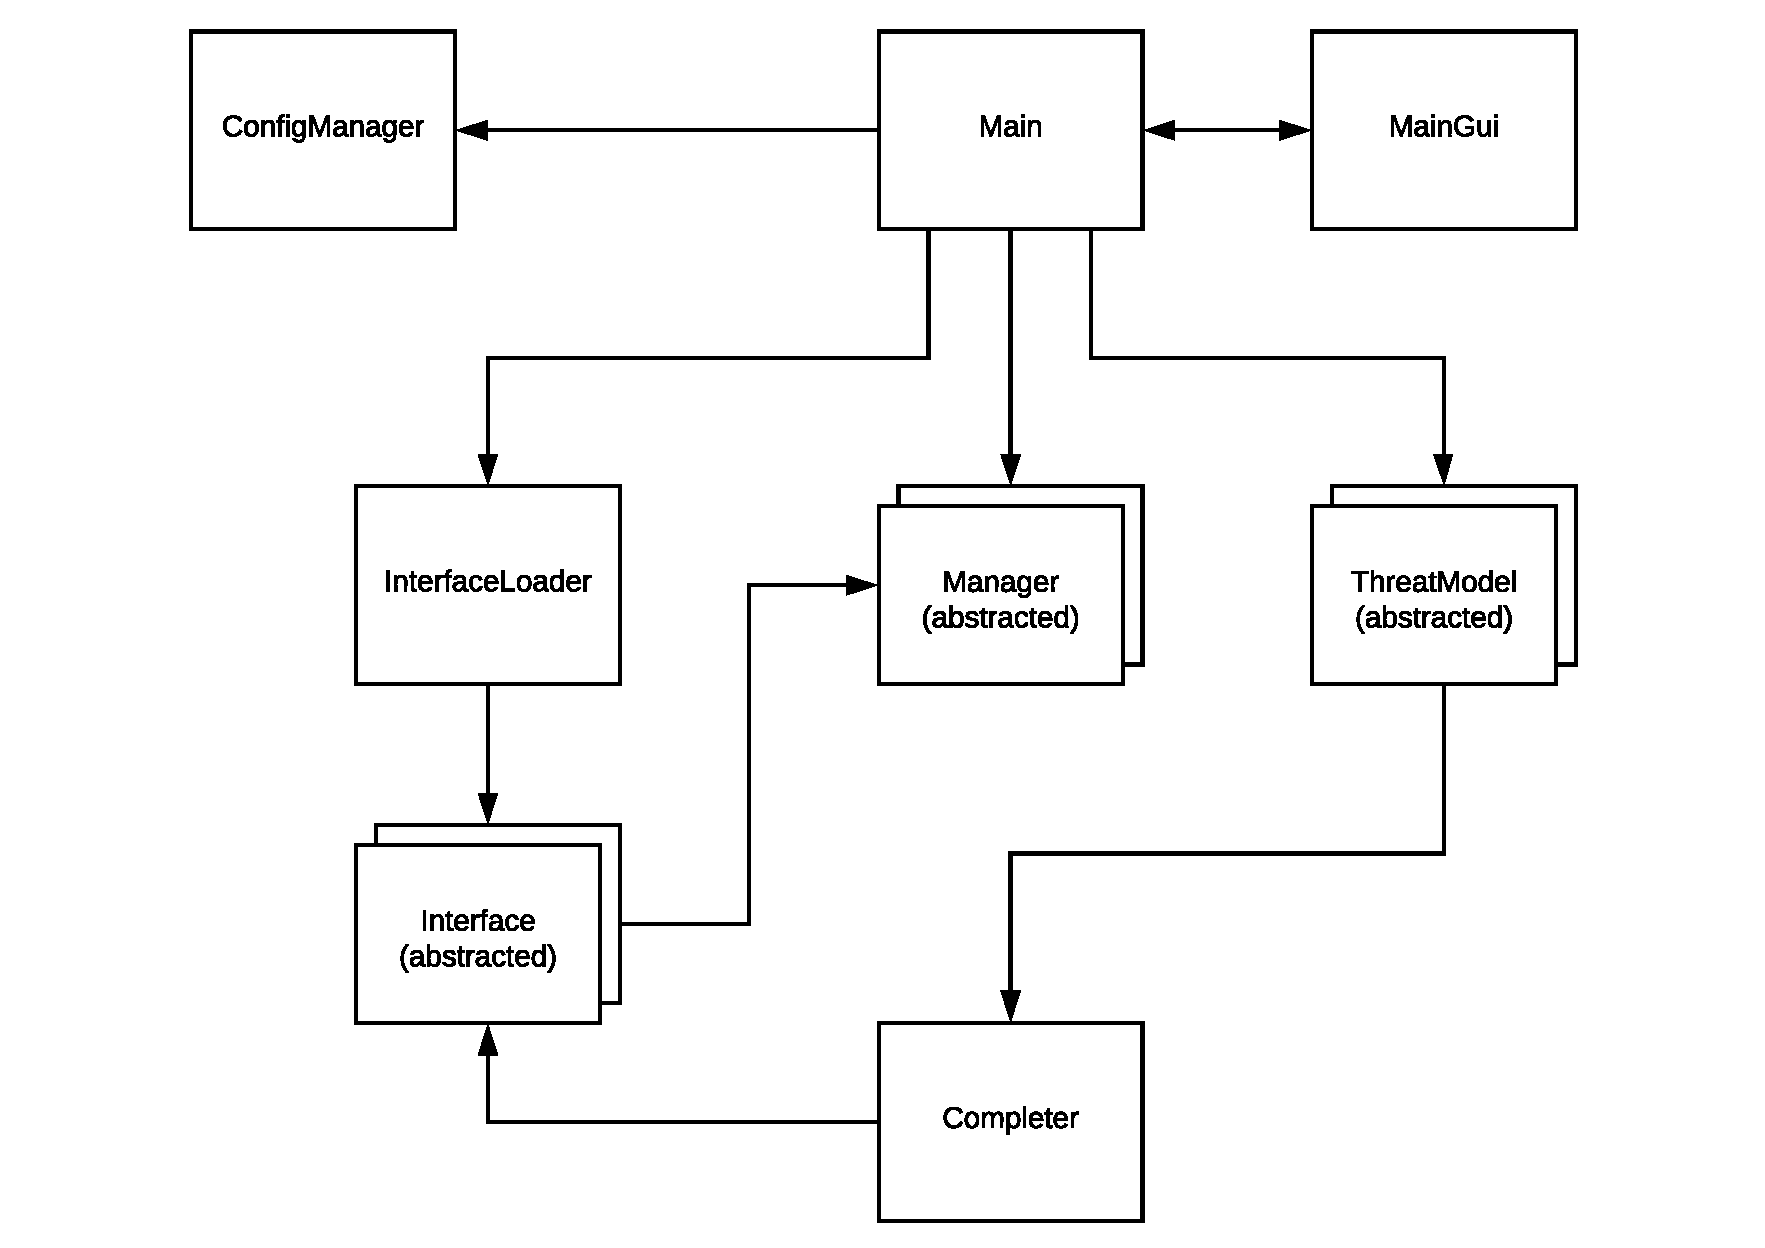
\includegraphics[width=\linewidth]
		{high_level_struct.pdf}}
	\caption{\label{fig:high-level-struct} High level project structure}
\end{figure}

It consists of two larger and four smaller parts. The "Main" and "MainGui" components represent application parent classes. They are responsible for configuration, initialization and start up. During startup phase "ConfigManager" is called to load global system configurations such as interface folder location and cache configuration. The "InterfaceLoader" object is one of the central parts of the application. It's purpose, as the name suggests, is to parse penetration tool configuration files and create tool "Interface" instances. "Manager" object supervises penetration tool execution and presents output.
"ThreatModel" object hides internal threat model complexity and governs it's display. "Completer" object is used to link threat model data with different penetration tools and their options. It generates input suggestions during pen testing sessions. 
"MainGui" object loads main parts of the GUI structure and controls threat model display.

Project layout diagram is provided in appendix \ref{sec:appendix-proj-struct}.


\subsubsection{Penetration tool interface}
Simplified penetration tool interface structure is presented in figure \ref {fig:interface-struct} below. \newline

\begin{figure}[!htb]
	\center{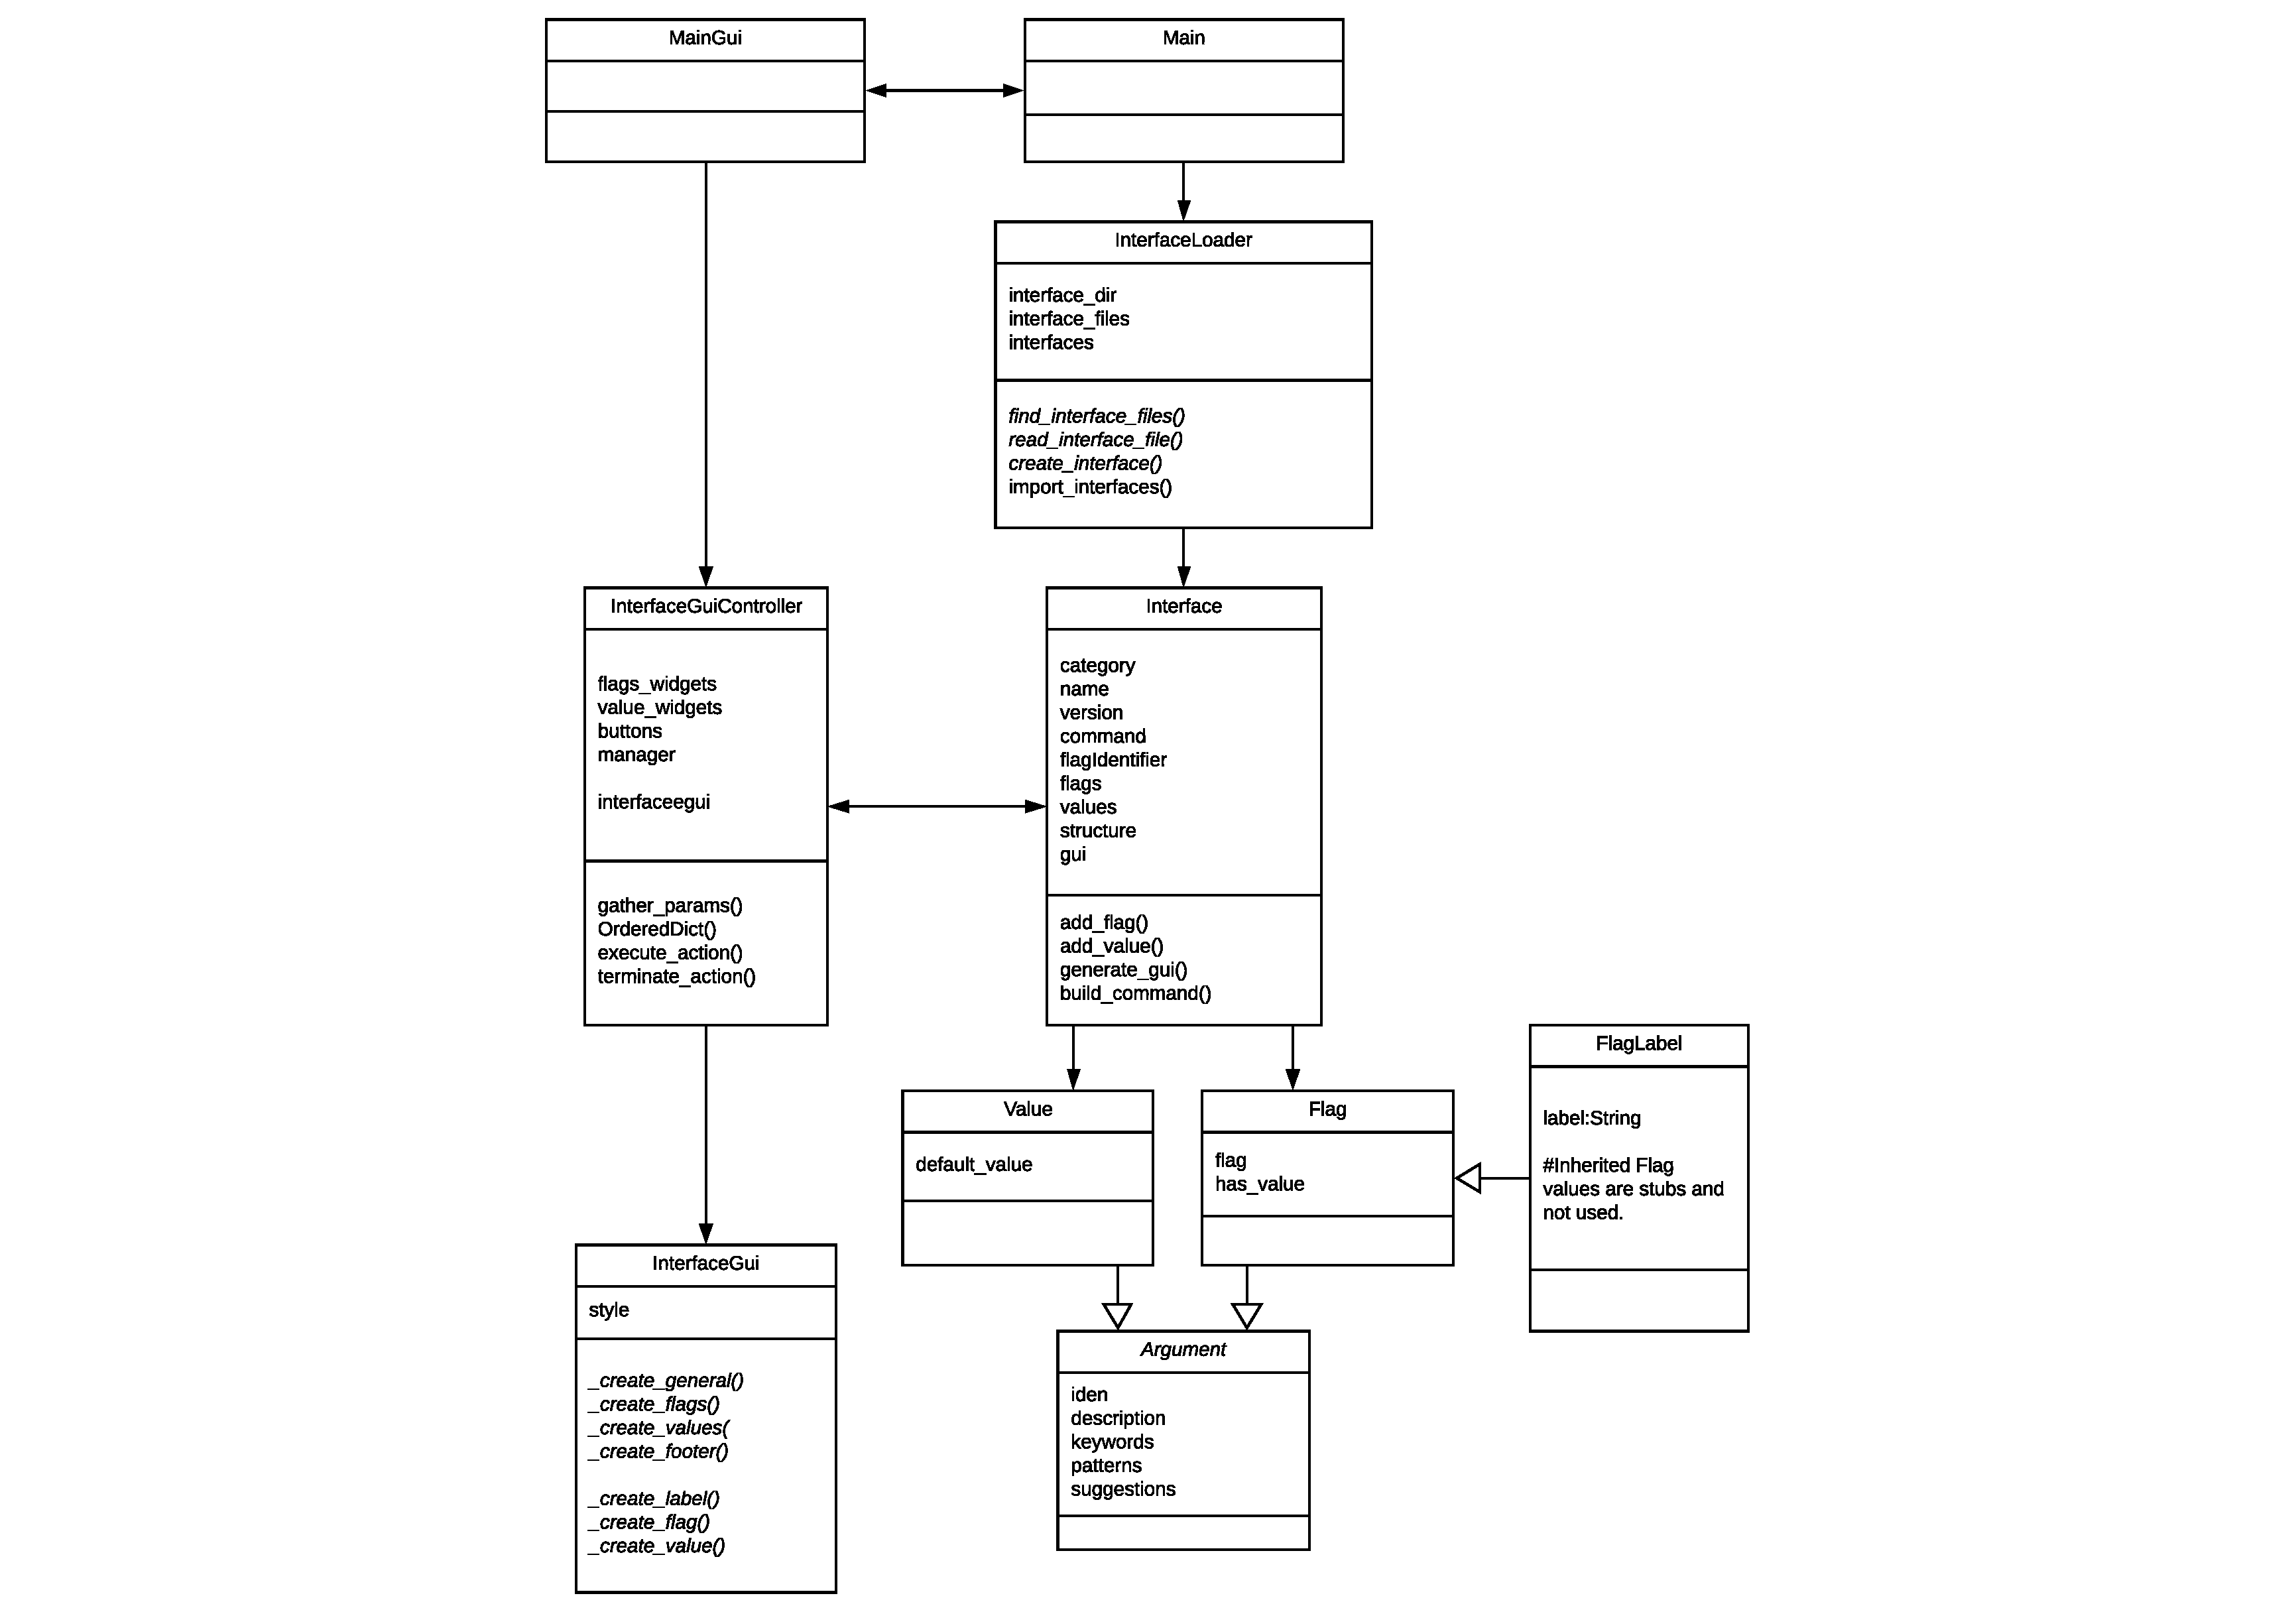
\includegraphics[width=1.7\linewidth]
		{interface_diagram.pdf}}
	\caption{\label{fig:interface-struct} Simplified penetration tool interface related project part}
\end{figure}

"InterfaceLoader" object is responsible for finding, parsing and storing added pen testing tool interfaces. Individual penetration tools are described using their configuration files, file structure example can be found in appendix \ref{sec:appendix-config-struct}. Configuration files define tools functionality and the way to map command line options to GUI entities. "Interface" objects are individual penetration tool representations in this project. "Interface" instances encapsulate overall penetration tool information required for it's use. Pen tool arguments are represented by the "Flag" and "Value" instances which are held in the "Instance" object. "FlagLabel" class is used to group "Flag" instances and as a visual marker in the GUI. 

Configuration parser design is recursive, thus "InterfaceLoader" only checks general configuration file structure. Similarly, "Interface" upon receiving data is only responsible for it's attributes, tool arguments are parsed by "Flag", "Value", "FlagLabel" and "Argument" classes accordingly. Distributed parsing reduces complexity and splits up responsibilities making verification and testing easier.

Interface GUI is structured following MVC pattern and is automatically generated from parsed attributes. This design supports nested tool parameters without any additional configuration. Although, out of projects scope, Qt library provide a markup language similar to CSS. Therefore, due to the recursive nature of the GUI design, only insignificant modifications would be needed to provide a neater user interface.


\subsubsection{Tool execution and output}
Simplified penetration tool execution and output display diagram is presented in figure \ref{fig:manager-struct} below.
\begin{figure}[!htb]
	\center{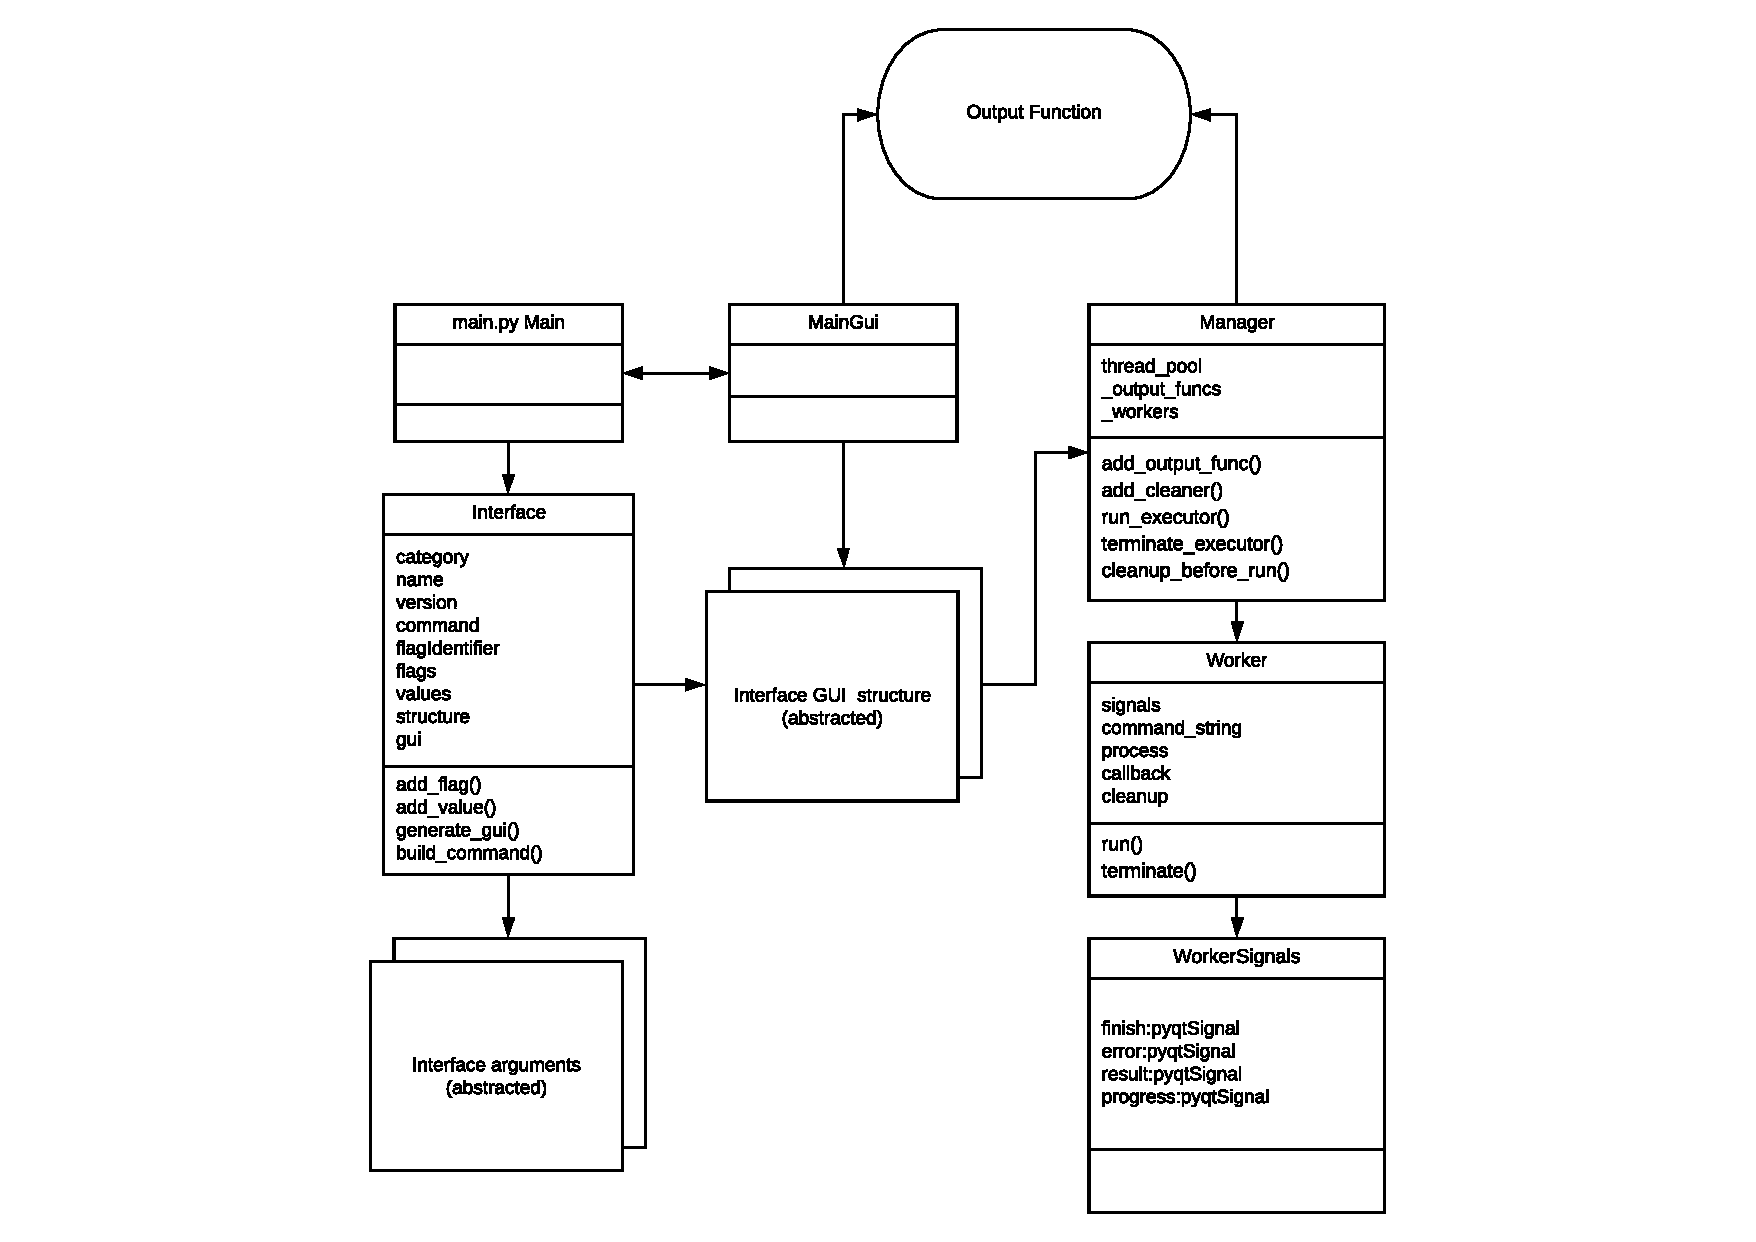
\includegraphics[width=1.3\textwidth]
		{manager_diagram.pdf}}
	\caption{\label{fig:manager-struct} Penetration tool execution}
\end{figure}

Individual pen tool (from now referred to as 'interface') execution is handled by the "Manager" object. Every interface GUI has a reference to the global "Manager" object. Upon every new interface GUI addition, a "MainGui" passes an "Output function" to the "Manager". The "Output functions" are mapped to individual interfaces inside the "Manager" object, after the interface execution they are called to display the results. Due to the variety of tools available and their visual output differences, the display functionality has been abstracted out from the system. Therefore, it is uncomplicated to extend the prototype with other ways of displaying the output. 

The "Manager" upon being given a command line string to creates a "Worker" instance which is responsible for it's execution. "Workers" start a new subprocess to run the command in the terminal. They can also receive updates on the process execution by the use of "WorkerSignals". "Manager" can be asked to terminate a command execution which by itself will send the termination signal to appropriate "Worker" object. When a "Worker" finishes the assigned task, it will use the "callback" function to notify the caller interface about task completion.

\subsubsection{Threat model representation}
Simplified proposed threat model implementation diagram is displayed in figure \ref{fig:threat-model-struct} below.\newline
IoT threat model described in "IoT Penetration Cookbook"\cite{cookbook} is implemented in the applications threat model section. The implementation uses MVC pattern and follows Single responsibility principle {19}. 

The threat model internal relations are abstracted using the "ThreatModel" object. As covered in the \ref{iot-threat-modelling} section, every IoT system is composed of "Assets", which are physical or virtual entities of the system. Every "Asset" can employ a number of technologies, in this design it would be more appropriate to say  that unique "Technologies" can be "used by" multiple "Assets". Every system contains multiple interaction points, here referred to as system "EntryPoints". Each "EntryPoint" is present in an "Asset". Potential system vulnerabilities are represented by the "Threat" objects. Each "Threat" is linked to a system "EntryPoint" and possible by exploiting some "Technologies" weaknesses. The individual "Threats" are then ranked using a ranking system - in this case DREAD, represented by the "DreadScore" object.

View and Controller parts are divided into multiple segments responsible only for the specific bit of GUI functionality. Threat model elements are organized using a tab menu where each tab content is generated by a different View object. Information displayed in the separate tabs is interconnected, therefore the observer pattern is used to keep it up to date. To make user interaction more convenient, the application remembers previously entered items making the GUI more user-friendly. The item 'caching' happens on system level, therefore, items from one threat model can be easily imported to another. Threat model front-end and back-end parts are connected view the parent "ThreatModelController" and ThreatModel" objects.


\begin{center}
	\begin{sideways}%[htbp]
		\begin{minipage}{\textheight}
			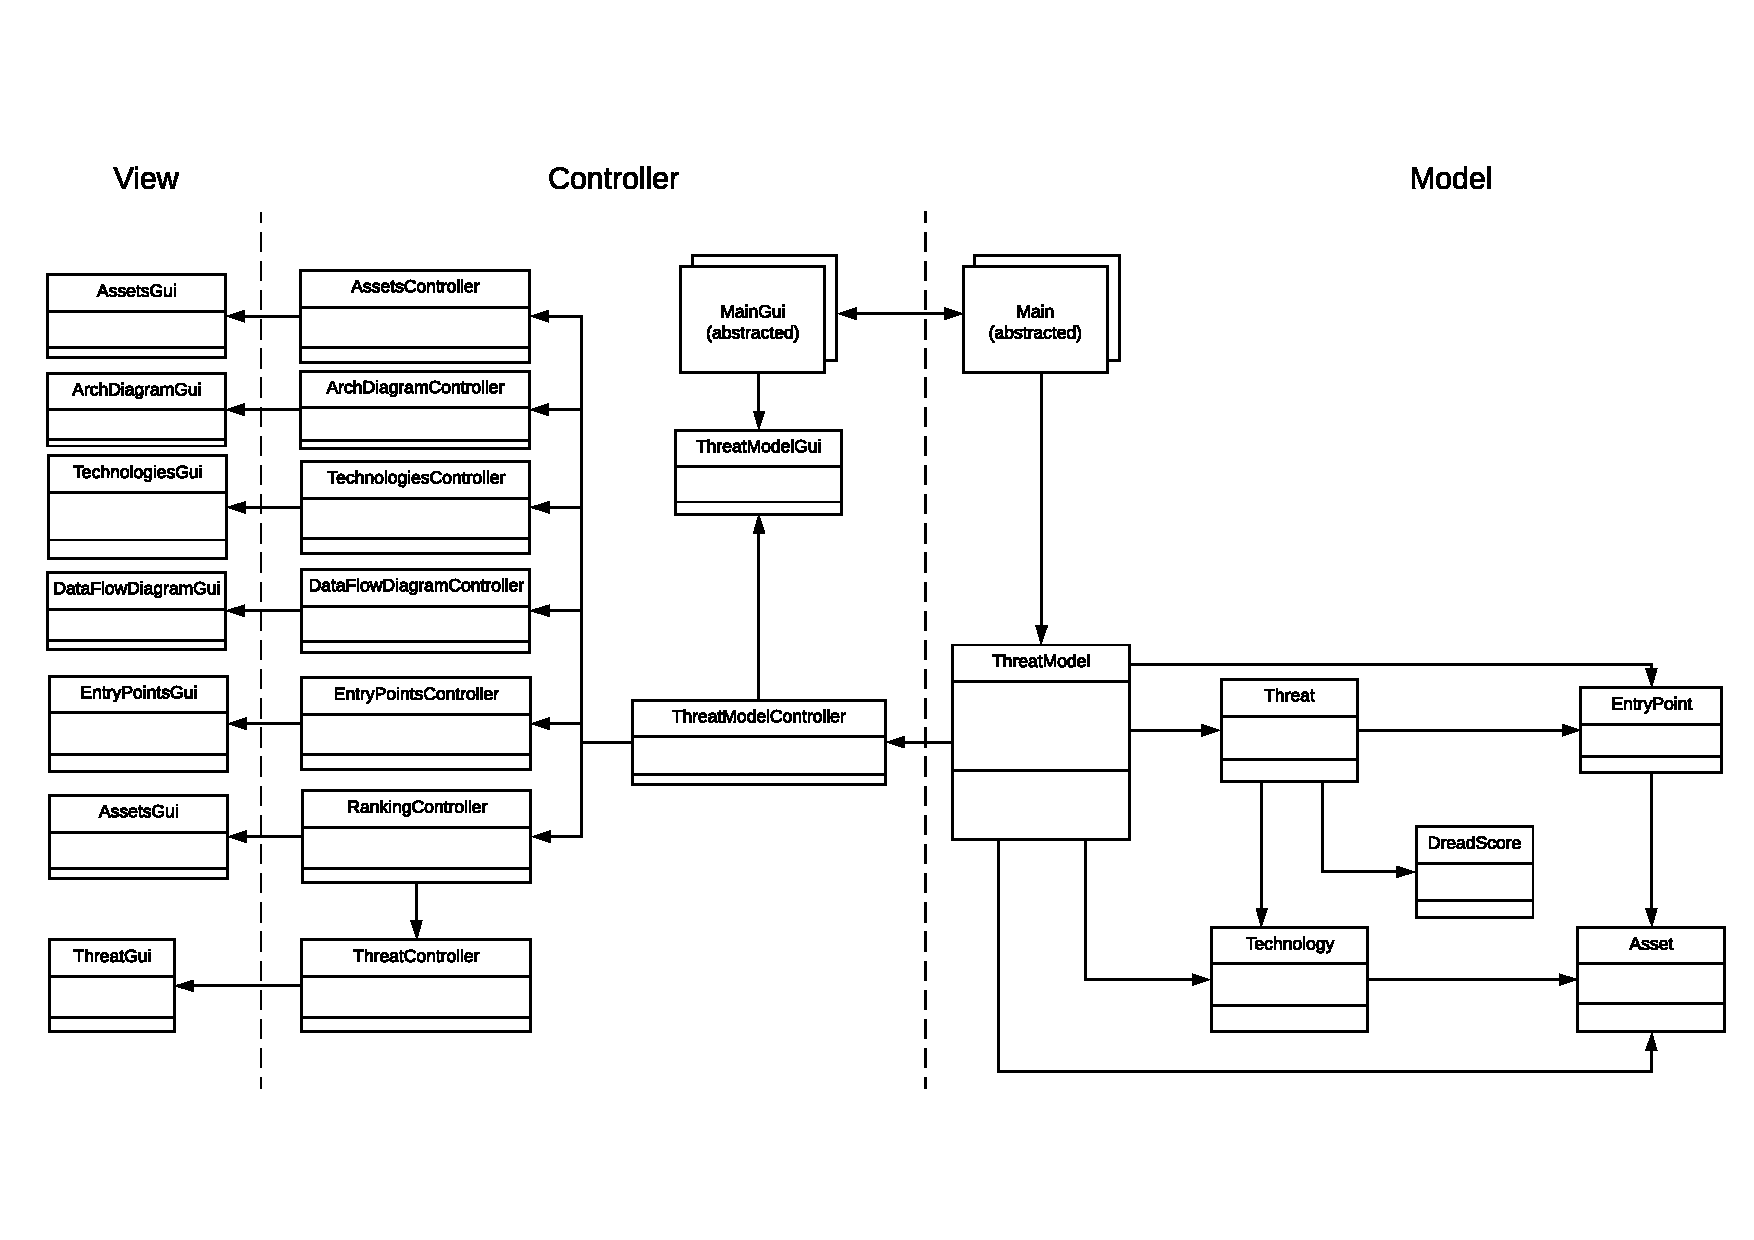
\includegraphics[width=\textwidth,keepaspectratio]{threat_model_diagram}
			\captionof{figure}{Threat Model structure}
			\label{fig:threat-model-struct}
		\end{minipage}
	\end{sideways}
\end{center}

\subsubsection{Suggestion generation}
Pen tool argument suggestion process diagram is presented in figure \ref{fig:completer} below.\newline
"Completer" object scans threat model data for specific words and phrases that match interface argument patterns. This functionality is provided as a convenience mechanism for the user linking threat model data with penetration tools included in the tool set. The "Completer" can only link keywords to assist pen testers work but at the current state can not suggest what kind of penetration test to use.

Interface configuration files can optionally contain "keywords" and "patterns" for every tool argument. These two sets of values can then be interpreted by "Completer" and matched to user entered values in the threat model. In order to separate threats information, completer requires a specific threat  to be selected from the threat list. This way information unrelated to that threat is filtered out. "Completer" works by scanning every "Threat" object attribute, then the "EntryPoint" object which is linked with that "Threat" instance, then the "Asset" object of the mentioned "EntryPoint", and finally "Technologies" suspected to be used by that "Threat".

In the pen tool GUI suggestions are presented as text completion drop down list, which helps to quickly entered values for the selected test. Only tool arguments that require the user to enter information by hand may have suggestions generated; boolean type command line arguments cannot have any values, therefore, suggestions model can not be applied to them. 

\begin{center}
	\begin{sideways}%[htbp]
		\begin{minipage}{\textheight}
			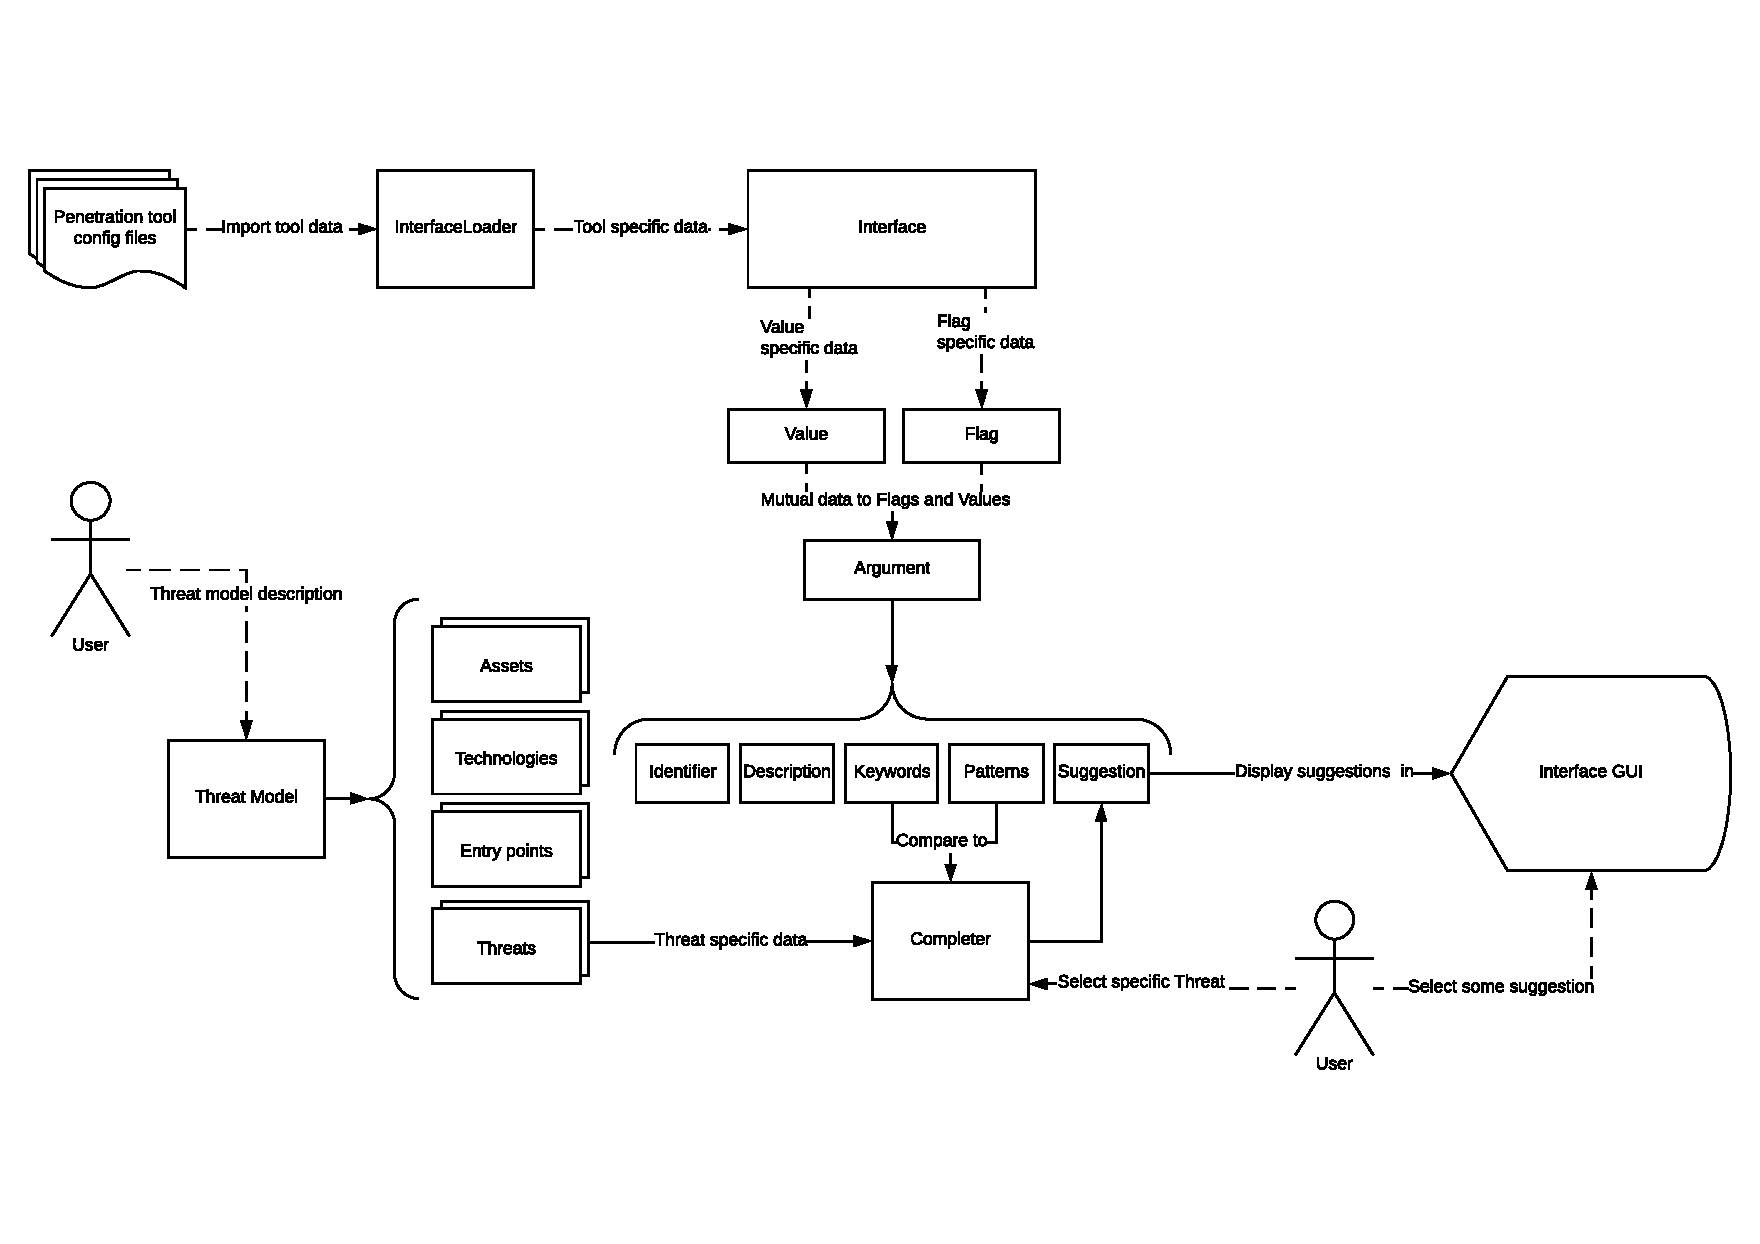
\includegraphics[width=\textwidth,keepaspectratio]{completer_diagram}
			\captionof{figure}{Suggestion generation control flow}
			\label{fig:completer}
		\end{minipage}
	\end{sideways}
\end{center}

